%%%%%%%%%%%%%%%%%%%% author.tex %%%%%%%%%%%%%%%%%%%%%%%%%%%%%%%%%%%
%
% sample root file for your "contribution" to a proceedings volume
%
% Use this file as a template for your own input.
%
%%%%%%%%%%%%%%%% Springer %%%%%%%%%%%%%%%%%%%%%%%%%%%%%%%%%%


\documentclass{svproc}

%%%%%%%%%%%%% Define various directories %%%%%%%%%%%%%%%%%%%%%%%%%%%%%%
\newcommand{\ResultsDirBase}{/home/jesse/Analysis/FemtoAnalysis/Results/}

%\newcommand{\ResultsDirBaseLamKch}{/home/jesse/Analysis/FemtoAnalysis/Results/Results_cLamcKch_20180505/}
%\newcommand{\ResultsDirBaseLamKs}{/home/jesse/Analysis/FemtoAnalysis/Results/Results_cLamK0_20180505/}
\newcommand{\ResultsDirBaseLamKch}{/home/jesse/Analysis/FemtoAnalysis/Results/Results_cLamcKch_20190319/}
\newcommand{\ResultsDirBaseLamKs}{/home/jesse/Analysis/FemtoAnalysis/Results/Results_cLamK0_20190319/}

\newcommand{\VZeroEffDirBase}{/home/jesse/Analysis/FemtoAnalysis/Results/V0Efficiency/}

\newcommand{\MomRes}{_MomResCrctn}%{}

%\newcommand{\NonFlatBgdLamKch}{_NonFlatBgdCrctnLamK0LinearLamKchPolynomial}
%\newcommand{\NonFlatBgdLamKs}{_NonFlatBgdCrctnLamK0LinearLamKchPolynomial}

\newcommand{\NonFlatBgdLamKch}{_NonFlatBgdCrctnLamK0LamKchPolynomial}
\newcommand{\NonFlatBgdLamKs}{_NonFlatBgdCrctnLamK0LamKchPolynomial}


\newcommand{\ResNum}{_3Res}
\newcommand{\PrimMaxDecay}{_PrimMaxDecay10fm}
\newcommand{\ResMethod}{_UsingXiDataAndCoulombOnly}

\newcommand{\ParamFixAndShareLamKch}{_ShareLam_Dualie_ShareLam_ShareRadii}
\newcommand{\ParamFixAndShareLamKs}{_ShareLam_Dualie_ShareLam_ShareRadii}

\newcommand{\SaveNameModLamKch}{\MomRes\NonFlatBgdLamKch\ResNum\PrimMaxDecay\ResMethod\ParamFixAndShareLamKch}
\newcommand{\SaveNameModLamKs}{\MomRes\NonFlatBgdLamKs\ResNum\PrimMaxDecay\ResMethod\ParamFixAndShareLamKs}


%%%%%%%% Shorthand definitions %%%%%%%%%%%%%%%%%%%%%%%%%%%%%%%%%%%%%%%%%%%%%%%%%%%%%%%%%%%%%
\newcommand{\kstar}{$k^{*}$\xspace}
\newcommand{\ktrue}{$k^{*}_{\mathrm{True}}$\xspace}
\newcommand{\krec}{$k^{*}_{\mathrm{Rec}}$\xspace}
\newcommand{\minv}{$m_{\mathrm{inv}}$\xspace}
\newcommand{\mt}{$m_{\mathrm{T}}$\xspace}
\newcommand{\pt}{$p_{\mathrm{T}}$\xspace}

\newcommand{\Lam}{$\mathrm{\Lambda}$\xspace}
\newcommand{\ALam}{$\overline{\mathrm{\Lambda}}$\xspace}
\newcommand{\LamALam}{$\mathrm{\Lambda}$ ($\overline{\mathrm{\Lambda}}$)\xspace}

\newcommand{\KchP}{$\mathrm{K^{+}}$\xspace}
\newcommand{\KchM}{$\mathrm{K^{-}}$\xspace}
\newcommand{\Kpm}{$\mathrm{K^{\pm}}$\xspace}

\newcommand{\Ks}{$\mathrm{K^{0}_{S}}$\xspace}

\newcommand{\LamK}{$\mathrm{\Lambda}\mathrm{K}$\xspace}
\newcommand{\ALamAK}{$\overline{\mathrm{\Lambda}}\overline{\mathrm{K}}$\xspace}


\newcommand{\LamKchP}{$\mathrm{\Lambda}\mathrm{K^{+}}$\xspace}
\newcommand{\ALamKchM}{$\overline{\mathrm{\Lambda}}\mathrm{K^{-}}$\xspace}
\newcommand{\LamKchPALamKchM}{$\mathrm{\Lambda}\mathrm{K^{+}}$ ($\overline{\mathrm{\Lambda}}\mathrm{K^{-}}$)\xspace}

\newcommand{\LamKchM}{$\mathrm{\Lambda}\mathrm{K^{-}}$\xspace}
\newcommand{\ALamKchP}{$\overline{\mathrm{\Lambda}}\mathrm{K^{+}}$\xspace}
\newcommand{\LamKchMALamKchP}{$\mathrm{\Lambda}\mathrm{K^{-}}$ ($\overline{\mathrm{\Lambda}}\mathrm{K^{+}}$)\xspace}

\newcommand{\LamKpm}{$\mathrm{\Lambda}\mathrm{K^{\pm}}$\xspace}
\newcommand{\ALamKpm}{$\overline{\mathrm{\Lambda}}\mathrm{K^{\pm}}$\xspace}
\newcommand{\LamALamKpm}{$\mathrm{\Lambda}$($\overline{\mathrm{\Lambda}}$)$\mathrm{K^{\pm}}$\xspace}


\newcommand{\LamKs}{$\mathrm{\Lambda}\mathrm{K^{0}_{S}}$\xspace}
\newcommand{\ALamKs}{$\overline{\mathrm{\Lambda}}\mathrm{K^{0}_{S}}$\xspace}
\newcommand{\LamKsALamKs}{$\mathrm{\Lambda}\mathrm{K^{0}_{S}}$ ($\overline{\mathrm{\Lambda}}\mathrm{K^{0}_{S}}$)\xspace}
\newcommand{\LamALamKs}{$\mathrm{\Lambda}$($\overline{\mathrm{\Lambda}}$)$\mathrm{K^{0}_{S}}$\xspace}

\newcommand{\XiKchP}{$\mathrm{\Xi}^{-}\mathrm{K^{+}}$\xspace}
\newcommand{\AXiKchM}{$\overline{\mathrm{\Xi}}^{+}\mathrm{K^{-}}$\xspace}

\newcommand{\XiKchM}{$\mathrm{\Xi}^{-}\mathrm{K^{-}}$\xspace}
\newcommand{\AXiKchP}{$\overline{\mathrm{\Xi}}^{+}\mathrm{K^{+}}$\xspace}


\newcommand{\XiKpm}{$\mathrm{\Xi}^{-}\mathrm{K^{\pm}}$\xspace}
\newcommand{\AXiKpm}{$\overline{\mathrm{\Xi}}^{+}\mathrm{K^{\pm}}$\xspace}

\newcommand{\Vz}{V$^{0}$\xspace}
%%%%%%%%%%%%%%%%%%%%%%%%%%%%%%%%%%%%%%%%%%%%%%%%%%%%%%%%%%%%%%%%%%%%%%%%%%%%%%%%%%%%%%%%%%%%

\usepackage{xspace}
\usepackage{multirow}
\usepackage{boldline}  % to make lines in table bold
\usepackage{comment}
\usepackage{graphicx,amsmath,amssymb,array,tabularx,url,xspace,subfigure}
\usepackage{relsize} %for \mathlarger
\usepackage{scalerel}  %to use scaleto functionality for math eqns (ex. in exponent of lambda eqn)
\usepackage{subfiles}
\usepackage{arrayjobx} % To use the array structures stored in FitResults_cLamcKch_20180505.tex 
\usepackage{wrapfig}

%
% RECOMMENDED %%%%%%%%%%%%%%%%%%%%%%%%%%%%%%%%%%%%%%%%%%%%%%%%%%%
%

% to typeset URLs, URIs, and DOIs
\usepackage{url}
\def\UrlFont{\rmfamily}

\begin{document}
\mainmatter              % start of a contribution
%
\title{\LamK femtoscopy in Pb--Pb collisions at $\mathbf{\sqrt{{\textit s}_{NN}}} =$ 2.76 TeV}

%
\titlerunning{\LamK femtoscopy in Pb--Pb collisions}  % abbreviated title (for running head)
%                                     also used for the TOC unless
%                                     \toctitle is used
%
\author{Jesse T. Buxton\inst{1} on behalf of the ALICE Collaboration}
%
\authorrunning{J.~T.~Buxton} % abbreviated author list (for running head)
%
%%%% list of authors for the TOC (use if author list has to be modified)

%
\institute{The Ohio Statue University, Columbus OH 43210, USA,\\
\email{jesse.thomas.buxton@cern.ch}}

\maketitle              % typeset the title of the contribution

\begin{abstract}
The first measurements of the scattering parameters of \LamK pairs in all three charge combinations (\LamKchP, \LamKchM, and \LamKs) are presented.
The results are achieved through a femtoscopic analysis of \LamK correlations in Pb--Pb collisions at $\sqrt{s_{\mathrm{NN}}}$ = 2.76 TeV recorded by ALICE at the LHC.  
The femtoscopic correlations result from strong final-state interactions, and are fit with a parametrization allowing for both the characterization of the pair emission source and the measurement of the scattering parameters for the particle pairs.
Extensive studies with the THERMINATOR 2 event generator provide a good description of the non-femtoscopic background, which result mainly from collective effects, with unprecedented precision.
Furthermore, this model together with HIJING simulations are used to account for contributions from residual correlations induced by feed-down from resonances.
The extracted scattering parameters indicate that the strong force is repulsive in the \LamKchP interaction and attractive in the \LamKchM and \LamKs interactions.
The results suggest an effect arising from different quark--antiquark interactions between the pairs ($\rm s\overline{s}$ in \LamKchP and $\rm u\overline{u}$ in \LamKchM), or from different net strangeness for each system (S=0 for \LamKchP, and S=$-2$ for \LamKchM).
Finally, the \LamK systems exhibit source radii larger than expected from extrapolation from identical particle femtoscopic studies.
This effect is interpreted as resulting from the separation in space--time of the single-particle \Lam and K source distributions.
\keywords{femtoscopy}
\end{abstract}
%


%************************************************************************************************************************
%************************************************************************************************************************
\section{Introduction}
\label{sec:Introduction}

Femtoscopy is an experimental method used to study the space--time characteristic of the particle emitting sources in relativistic particle collisions~\cite{Lisa:2005dd}.  
With this method, two- (or many-) particle relative-momentum correlation functions are used to connect the final-state momentum distributions to the space--time distributions of particle emission at freeze-out.  
Current femtoscopic studies are able to extract the size, shape, and orientation of the pair emission regions, as well as offer estimations of the total time to reach kinetic decoupling and the suddenness of particle emission~\cite{Lisa:2005dd,Lisa:2008gf}.
The correlation functions are sensitive to quantum statistics, as well as strong and Coulomb final-state interactions (FSI).  
Thus, in addition to characterizing the source region, femtoscopy offers a unique environment in which to measure nuclear scattering parameters, many of which are difficult, if not impossible, to measure otherwise.  


The first measurements of the scattering parameters of \LamK pairs in all three charge combinations (\LamKchP, \LamKchM, and \LamKs) are presented.
The scattering parameters, along with pair emission source sizes, are extracted with a femtoscopic analysis of \LamK correlations for three centrality percentile ranges (0--10\%, 10--30\%, and 30--50\%) in Pb--Pb collisions at $\sqrt{s_{\mathrm{NN}}}$ = 2.76 TeV measured by the ALICE experiment at the LHC.  
These correlations result from strong final-state interactions, and are fit with a parametrization by Lednick\'y and Lyuboshitz~\cite{Lednicky:82}.  
Extensive studies with the THERMINATOR 2 event generator are performed to account for both non-femtoscopic backgrounds, as well as contributions from residual correlations induced by feed-down from resonances.

Throughout the text, the pair name is used as shorthand for the pair-conjugate system, which are found to be consistent (e.g., \LamKchP for \LamKchP $\oplus$ \ALamKchM, \LamKchM for \LamKchM $\oplus$ \ALamKchP, and \LamKs for \LamKs $\oplus$ \ALamKs), and \LamK is used to describe all \LamK combinations.


%************************************************************************************************************************
%************************************************************************************************************************
\section{Data analysis}
\label{sec:DataAnalysis}

This work reports on the analysis of Pb--Pb collisions at $\sqrt{s_{\mathrm{NN}}}$ = 2.76 TeV produced by the LHC and measured by the ALICE experiment~\cite{Aamodt:2008zz} in 2011.
In order for an event to be included in the analysis, the $z$ position of the reconstructed event vertex must be within 10 cm of the center of the ALICE detector. 
Charged particle tracking was performed using the Time Projection Chamber (TPC)~\cite{2010NIMPA.622..316A} and the Inner Tracking System~\cite{Abelevetal:2014dna}.  
Particle identification (PID) for reconstructed tracks was carried out using both the TPC and Time-Of-Flight (TOF) detectors~\cite{Abelev:2014ffa,Akindinov:2013tea} in the pseudorapidity range $|\eta| < 0.8$.  

%************************************************************************************************************************
%%\subsection{K$^{\pm}$ selection}
%%\label{sec:KchSelection}
Tracks reconstructed for the charged kaon samples were required to be within the range 0.14 $<$ \pt $<$ 1.5 GeV/$c$.
To reduce the number of secondary particles (e.g., charged particles produced in the detector material, particles from weak decays, etc.) in the samples, distance-of-closest-approach (DCA) of the track to the primary vertex was required to be less than 2.4 cm in the transverse direction and less than 3.0 cm in the longitudinal direction.
Particle identification was performed using both the TPC and TOF detectors via the $N_{\sigma}$ method. 
The $N_{\sigma}$ selection criteria become tighter with increasing momentum to reduce contamination within the samples, as the \Kpm signals begin to overlap more significantly with those from other particles, particularly e$^{\pm}$ and $\pi^{\pm}$.
Additional methods are included to reduce the contamination in the \Kpm samples from the electrons and pions.  
The purity of the \Kpm collections, $P_{\mathrm{K}^{\pm}}$, was estimated to be approximately 97\% from a Monte-Carlo (MC) study based on HIJING~\cite{PhysRevD.44.3501} simulations using GEANT3~\cite{Brun:1082634} to model particle transport through the ALICE detectors. 
For a more detailed estimate of the \Kpm purity from an analysis employing similar methods, see~\cite{Acharya:2017qtq}.


%************************************************************************************************************************
%%\subsection{\Vz selection}
%%\label{sec:V0Selection}

Electrically neutral \LamALam and \Ks particles are reconstructed through their weak decays: \Lam $\rightarrow$ p$\pi^{-}$ (\ALam $\rightarrow \pi^{+}\overline{\mathrm{p}}$) and \Ks $\rightarrow$ $\pi^{+}\pi^{-}$.
The obtained candidates are denominated as \Vz particles.
Aside from typical kinematic and PID selection methods (using TPC and TOF detectors), the tracks of the decay products (called \textit{daughters}) are also exposed to a minimum requirement of their impact parameter with respect to the primary vertex.  
To help ensure quality, a maximum value is demanded on the distance of closest approach between the daughters.
To select primary candidates, the impact parameter with respect to the primary vertex is used as a selection criterion for each \Vz.
Furthermore, a restriction is imposed on the pointing angle, $\theta_{\mathrm{PA}}$, between the \Vz momentum and the vector pointing from the primary vertex to the secondary \Vz decay vertex, which is achieved by appointing a minimum value on $\cos(\theta_{\mathrm{PA}})$.
A method was implemented to remove the contamination to the \LamALam and \Ks samples due to misidentification of the protons and pions for each \Vz.
A final restriction on the invariant mass (\minv) is applied to enhance the purity.
To avoid any auto-correlation effects, all \Vz candidates within each single-particle collection (\Lam, \ALam, and \Ks separately) are ensured to have unique daughters. 
The \Lam and \ALam purities are estimated to be $P_{\Lambda(\overline{\Lambda})} \approx 95\%$, and that of the \Ks is $P_{\mathrm{K^{0}_{S}}} \approx 98\%$.


%************************************************************************************************************************
%%\subsection{Pair construction}
%%\label{PairConstruction}

When forming particle pairs, a shared daughter restriction is applied to ensure the first particle in the pair is unique from the second. 
This is implemented by removing all \LamKs pairs which share a daughter, and removing all \LamKpm pairs in which the \Kpm track is also claimed as a daughter of the \Lam.
Furthermore, an average separation constraint is imposed to remove splitting and merging effects, in which the average separation between two tracks is calculated using their spatial separation as determined at several points throughout the TPC.
For the \LamKs analysis, a minimum average separation constraint of 6 cm between the like-charge daughters in the pairs is imposed.
For the \LamKpm analyses, a minimum average separation constraint of 8 cm is enforced between the \Kpm and the \Lam daughter with like charge.

%************************************************************************************************************************
%************************************************************************************************************************
\section{Analysis methods}
\label{sec:AnalysisMethods}

%************************************************************************************************************************
\subsection{Correlation function}
\label{sec:CorrelationFunction}
The two-particle correlation function for particles $a$ and $b$, $C_{ab}(\vec{\mathrm{p}}_{a},\vec{\mathrm{p}}_{b})$, is defined as the ratio of the probability of simultaneously measuring two particles with momenta $p_{a}$ and $p_{b}$, to the product of the single-particle probabilities.
These probabilities are directly related to the covariant two-particle spectrum, $E_{a}E_{b}\frac{dN_{ab}}{d^{3}p_{a}d^{3}p_{b}}$, and the single-particle spectra, $E_{a(b)}\frac{dN_{a(b)}}{d^{3}p_{a(b)}}$, and the correlation function may be written
\begin{equation}
  C_{ab}(\vec{\mathrm{p}}_{a},\vec{\mathrm{p}}_{b}) = \frac{E_{a}E_{b}\frac{dN_{ab}}{d^{3}p_{a}d^{3}p_{b}}}{\big( E_{a}\frac{dN_{a}}{d^{3}p_{a}} \big) \big( E_{b}\frac{dN_{b}}{d^{3}p_{b}} \big)},
\label{eqn:CfRatioSpectra}
\end{equation}
where $N_{ab}$ is the yield of particle pairs, $E_{a(b)}$ is the energy, $p_{a(b)}$ is the three-momentum, and $N_{a(b)}$ is the yield of particles $a(b)$.
Theoretically, the correlation function may be expressed as in the Koonin-Pratt equation~\cite{Koonin:1977fh,Pratt:1990zq},
\begin{equation}
 C(\mathbf{k^{*}}) = \int S_{\mathbf{P}}(\mathbf{r^{*}})|\mathrm{\Psi}_{\mathbf{k^{*}}}(\mathbf{r^{*}})|^{2}d^{3}\mathbf{r^{*}},
\label{eqn:KooninPrattEqn}
\end{equation}
where $\mathbf{k}^{*}$ is the relative momentum of the pair (defined as $\mathbf{k}^{*} = \frac{1}{2}|\mathbf{p}_{1}^{*}-\mathbf{p}_{2}^{*}|$, where $\mathbf{p}_{1}^{*}$ and $\mathbf{p}_{2}^{*}$ are the momenta of the two particles) in the pair rest frame (PRF), $\mathbf{r}^{*}$ is the relative separation in the same frame, $\mathbf{P}$ is the total pair momentum, $S_{\mathbf{P}}(\mathbf{r^{*}})$ is the pair source distribution, and $\mathrm{\Psi}_{\mathbf{k^{*}}}(\mathbf{r^{*}})$ is the two-particle wave-function.
Within the $|\mathrm{\Psi}|^{2}$ term the particle interaction information is contained, and therefore the scattering parameters.

In practice, the correlation function is formed experimentally as $C(k^{*}) = \mathcal{N}\frac{A(k^{*})}{B(k^{*})}$, where $A(k^{*})$ is the signal distribution, $B(k^{*})$ is the reference distribution, and $\mathcal{N}$ is a normalization parameter.  
The reference distribution is used to divide out the phase-space effects, leaving only the femtoscopic effects in the correlation function. 
The normalization parameter is chosen such that the mean value of the correlation function equals unity for \kstar $\in$ [0.32, 0.4] GeV/$c$.
The signal distribution is the same-event distribution of particle pairs.
The reference distribution is obtained using mixed-event pairs~\cite{Kopylov:1974th}, i.e., particles from a given event are paired with those from another event.
In order to mix similar events, only events of like centrality (within 5\%) and of like primary vertex position (within 2 cm) are mixed.

%************************************************************************************************************************
\subsection{Modeling the correlation function}
\label{sec:ModelingCF}

In the absence of the Coulomb interaction, the correlation function can be described analytically with a model derived by Lednick\'y and Lyuboshitz~\cite{Lednicky:82},
\begin{equation}
\begin{aligned}
C(k^{*})_{\mathrm{Lednick\acute{y}}} = &1 + \sum_{S}\rho_{S}\left[\frac{1}{2}\left|\frac{f^{S}(k^{*})}{R_{\mathrm{inv}}}\right|^2\left(1-\frac{d^{S}_{0}}{2\sqrt{\pi}R_{\mathrm{inv}}}\right) \right. \\
&+ \left. \frac{2\Re f^{S}(k^{*})}{\sqrt{\pi}R_{\mathrm{inv}}}F_{1}(2k^{*}R_{\mathrm{inv}})-\frac{\Im f^{S}(k^{*})}{R_{\mathrm{inv}}}F_{2}(2k^{*}R_{\mathrm{inv}})\right],
\end{aligned}  
\label{eqn:LednickyEqn}
\end{equation}
where $\Re f(k^{*})$ and $\Im f(k^{*})$ denote the real and imaginary parts of the complex scattering amplitude, respectively, $F_{1}$ and $F_{2}$ are the analytic functions, and $R_{\mathrm{inv}}$ is the radius of the spherically symmetric Gaussian distribution assumed for the pair emission source in the PRF.
The complex scattering amplitude is evaluated via the effective range approximation,
\begin{equation}
\begin{aligned}
f(k^{*}) = \left( \frac{1}{f_{0}} + \frac{1}{2}d_{0}k^{*2} - ik^{*} \right)^{-1},
\end{aligned}
\label{eqn:ScatteringParam}
\end{equation}
where $f_{0}$ is the complex s-wave scattering length, $d_{0}$ is the effective range of the interaction.
The sign convention is such that a positive real component of the scattering length, $\Re f_{0}$, represents an attractive interaction, while a negative $\Re f_{0}$ represents a repulsion.



%************************************************************************************************************************
\subsection{Residual correlations}
\label{ResidualCorrelations}

Femtoscopic analyses are sensitive to the pair emission structure at kinetic freeze-out. Therefore, within
femtoscopy, any particle which originates from a resonance decay before last rescattering is considered
primary.

In practice, some of the selected particles originate as decay products from other resonances, and some of the final pairs contain a misidentified member.
The contributions from fake pairs, which contain at least one misidentified member, are assumed to average to unity, in which case they simply attenuate the femtoscopic signal.
The main sources of residual correlations in the \LamK systems result from \Lam hyperons which have decayed from $\mathrm{\Sigma}^{0}$, $\mathrm{\Xi}^{0}$, and $\mathrm{\Xi}^{-}$ parents.
The finally measured correlation function is a combination of the genuine \LamK correlation with contributions from resonances and impurities~\cite{Kisiel:2014mma},
\begin{equation}
\begin{aligned}
\label{eqn:CfwRes} 
 C_{\mathrm{measured}}(k^{*}_{\Lambda\mathrm{K}}) &= 1 + \lambda'_{\Lambda\mathrm{K}}[C_{\Lambda\mathrm{K}}(k^{*}_{\Lambda\mathrm{K}}) - 1] + \sum\limits_{ij}  \lambda'_{ij}[C_{ij}(k^{*}_{\Lambda\mathrm{K}})-1], \\
\end{aligned} 
\end{equation}
with
\begin{equation}
\begin{aligned}
\label{eqn:CfwRes2} 
 \lambda_{ij}' &= \lambda_{\mathrm{Fit}}\lambda_{ij}, \\
 \sum\limits_{ij}\lambda_{ij}' &=  \lambda_{\mathrm{Fit}}\sum\limits_{ij}\lambda_{ij} = \lambda_{\mathrm{Fit}},
\end{aligned} 
\end{equation}
where the \LamK term represents the genuine \LamK correlation, and the $ij$ terms denote the contributions from residual correlations resulting from feed-down and impurities.
More specifically, $C_{ij}(k^{*}_{\Lambda\mathrm{K}})$ is the correlation function of the parent system expressed in terms of the relative momentum of the daughter \LamK pair.  
The $\lambda_{ij}$ parameters serve as weights dictating the relative strength of each component's contribution to the observed signal, are estimated using the THERMINATOR 2 and HIJING simulations, and are normalized to unity (i.e., $\sum_{ij} \lambda_{ij} = 1$, where $ij$ includes also the primary \LamK component)~\cite{Kisiel:2014mma,Acharya:2018gyz}.

Since the interactions between these particles are not known, some assumptions must be made.
When modeling the parent systems, the source radii are assumed to be equal to those of the daughter \LamK systems.
Furthermore, Coulomb-neutral parent pairs are assumed to share the same scattering parameters as the \LamK daughter pair, and the parent correlation function is modeled using Eq.~\ref{eqn:LednickyEqn}.
During the fit process, these source radii and scattering parameters are left free, as described in Sec.~\ref{SummarizedFitProcedure}.
For the \XiKpm parent system, where the constituents interact via both the strong and Coulomb interactions, no analytical expression exists to model the correlation function (see App.~\ref{App:CoulombFitter}), and the experimental \XiKpm data are used.


To obtain the parent correlation function expressed in the relative momentum of the daughter pair, a transform matrix is utilized,
\begin{equation}
  C_{ij}(k^{*}_{\Lambda\mathrm{K}}) \equiv \frac{\sum\limits_{k^{*}_{ij}} C_{ij}\left(k^{*}_{ij}\right) T\left(k^{*}_{ij},k^{*}_{\Lambda\mathrm{K}}\right)}{\sum\limits_{k^{*}_{ij}} T\left(k^{*}_{ij},k^{*}_{\Lambda\mathrm{K}}\right)},
\label{eqn:ResidualsTransform}
\end{equation}
where $T(k^{*}_{ij},k^{*}_{\Lambda\mathrm{K}})$ is the transform matrix, which is generated with the THERMINATOR 2~\cite{Chojnacki:2011hb} simulation. 
The transform matrix describes the decay kinematics of the parent system into the daughter, and is essentially an unnormalized probability distribution mapping the \kstar of the parent pair to that of the daughter pair when one or both parents decay (see~\cite{Kisiel:2014mma} for more details).

%************************************************************************************************************************
\subsection{Non-femtoscopic background}
\label{NonFlatBackground}

A significant non-femtoscopic background is observed in all of the studied \LamK correlations, which increases with decreasing centrality, is the same amongst all \LamKpm pairs, and is more pronounced in the \LamKs system (the difference in \LamKpm and \LamKs backgrounds is due mainly to a difference in kinematic selection criteria).  
The background is primarily due to particle collimation associated with elliptic flow, and results from mixing events with unlike event planes~\cite{Kisiel:2017}.
The effect produces the observed suppression at intermediate \kstar, and should also lead to an enhancement at low \kstar.
The behavior of the non-femtoscopic background is needed in the low \kstar femtoscopic signal region, but an isolated view of it is only possible outside of such a region.

The THERMINATOR 2 simulation has been shown to reproduce the background features in a $\pi$K analysis~\cite{Kisiel:2017}. 
The simulation does not include any final-state effects, but they can be introduced by weighting the numerator pairs with the modulus squared of the appropriate two-particle wave-function when building the signal distributions. 
For the present purpose, only the behavior of the non-femtoscopic background is desired, and unit weights are used.
Figure~\ref{fig:BgdswTHERM} shows the THERMINATOR 2 simulation together with experimental data.  
The figure also shows a 6$^{\mathrm{th}}$-order polynomial fit to the simulation, as well as the fit polynomial scaled to match the data.

The THERMINATOR 2 simulation offers a good description of the non-femtoscopic backgrounds in the \LamK systems, and can be used in a quantitative fashion to help fit the data.
More specifically, the non-femtoscopic backgrounds are modeled by 6$^{\mathrm{th}}$-order polynomial fits to THERMINATOR 2 simulation,
\begin{equation}
F_{\scaleto{THERM.\; Bgd}{6pt}}(k^{*}) = a{k^{*}}^{6}+ b{k^{*}}^{5} + c{k^{*}}^{4} + d{k^{*}}^{3} + e{k^{*}}^{2} + fk^{*} + g,
\end{equation}
where the linear term coefficient is fixed to zero ($f=0$), and one polynomial is fit for each centrality class and \LamK charge combination.
The coefficients of each polynomial are set before application with the experimental data by fitting to the THERMINATOR 2 simulation, shown in Fig.~\ref{fig:BgdswTHERM}.
The extracted polynomial is adjusted to best describe the experimental data by introducing a scale factor and a vertical shift,
\begin{equation}
F_{\scaleto{Bgd}{6pt}}(k^{*}) = \alpha\cdot F_{\scaleto{THERM.\; Bgd}{6pt}}(k^{*}) + \beta,
\end{equation}
where $\alpha$ and $\beta$ are determined by fitting to the data in the region $0.32 < k^{*} < 0.80$ GeV/$c$; during the fit of the low-\kstar signal region, the background is fixed.
In all cases, the non-femtoscopic background correction was applied as a scale factor.


\begin{figure}[h]
  \centering
  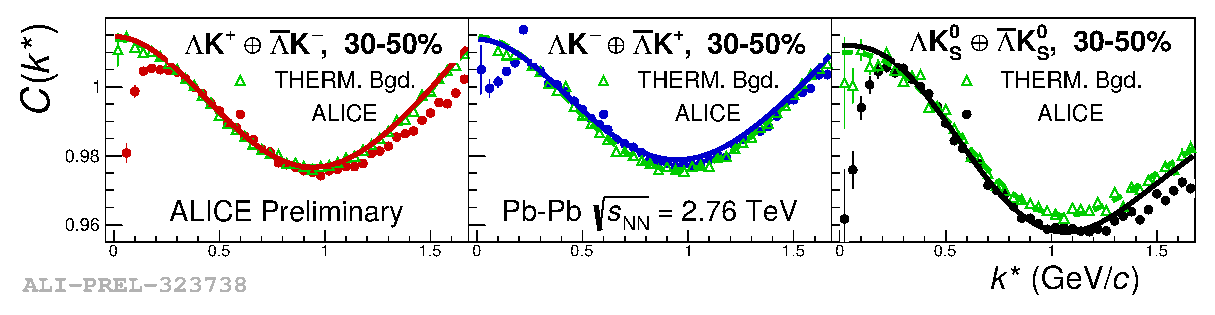
\includegraphics[width=\textwidth]{./Figures/Approved/OtherFormats/EPS/2019-06-11-BgdwFitOnly_RandomEPs_NumWeight1_Full_AllAnwConj_3050.eps}
  \caption[Backgrounds with THERMINATOR 2]
  {
  (Color online) THERMINATOR 2 simulation (open squares) together with experimental data (closed circles) for the 30--50\% centrality percentile range.  
  Results are shown for \LamKchP (left), \LamKchM (middle), and \LamKs (right).
  A $6^{\mathrm{th}}$-order polynomial fit to the simulation is shown as a dashed curve.  
  This polynomial is scaled to match the experimental data.  
  The polynomial fit with scale factor applied is drawn as a solid curve.
  }
  \label{fig:BgdswTHERM}
\end{figure} 


%************************************************************************************************************************
\subsection{Summarized correlation function construction}
\label{SummarizedFitProcedure}

The parameters included in the generation of a correlation function are: $\lambda_{\mathrm{Fit}}$, $R$, $f_{0}$ ($\Re f_{0}$ and $\Im f_{0}$ separately), $d_{0}$, and normalization $\mathcal{N}$.
For the fit, a given pair and its conjugate (e.g., \LamKchP and \ALamKchM) share scattering parameters ($\Re f_{0}$, $\Im f_{0}$, $d_{0}$), and the three distinct analyses (\LamKchP, \LamKchM, and \LamKs) are assumed to have scattering parameters unique from each other.
The pair emission source for a given centrality class is assumed similar among all analyses; therefore, for each centrality, all \LamK analyses share a common radius parameter.
For each centrality class, a single $\lambda_{\mathrm{Fit}}$ parameter (see Eq.~\ref{eqn:CfwRes}) is shared amongst all.
Finally, each correlation function has a unique normalization parameter, $\mathcal{N}$.

All experimental correlation functions are normalized in the range 0.32 $< k^{*} <$ 0.40 GeV/$c$, and fit in the range 0.0 $< k^{*} <$ 0.30 GeV/$c$.
For the \LamKchM analysis, the region 0.19 $< k^{*} <$ 0.23 GeV/$c$ was excluded from the fit to exclude the bump caused by the $\Omega^{-}$ resonance.
For each pair system, contributions from three residual contributors are accounted for, as discussed in Sec.~\ref{ResidualCorrelations}, and whose individual $\lambda$ values are listed in Table~\ref{tab:LambdaValues_3Res}.
Effects of finite track momentum resolution are also accounted for, as outlined in Sec.~\ref{MomentumResolutionCorrections}.
The non-femtoscopic backgrounds are modeled using the THERMINATOR 2 simulation, as described in Sec.~\ref{NonFlatBackground}.
A log-likelihood fit function is used as the statistic quantifying the quality of the fit~\cite{Lisa:2005dd}.

To summarize, the complete fit function is constructed as follows.
The uncorrected, primary, correlation function, $C_{\Lambda\mathrm{K}}(k^{*}_{\mathrm{\Lambda K,\,True}})$, is constructed using Eq.~\ref{eqn:LednickyEqn}.
The correlation functions describing the parent systems which contribute residually, $C_{ij}(k^{*}_{ij,\,\mathrm{True}})$, are obtained using Eq.~\ref{eqn:LednickyEqn} for Coulomb-neutral pairs or experimental data for \XiKpm contributions.
The residual contributions are then found by running each parent correlation function through the appropriate transform matrix, via Eq.~\ref{eqn:ResidualsTransform}.
The primary and residual correlations are combined, via Eq.~\ref{eqn:CfwRes} with Tab.~\ref{tab:LambdaValues_3Res}, to form $C'_{Fit}$(\ktrue).
Corrections are applied to account for momentum resolution effects using Eq.~\ref{eqn:MomResCorrection}, to obtain $C'_{\mathrm{Fit}}(k^{*}_{\mathrm{Rec}})$.
Finally, the non-femtoscopic background correction, $F_{\mathrm{Bgd}}(k^{*}_{\mathrm{Rec}})$, is applied and the final fit function is obtained,
\begin{equation}
C_{\mathrm{Fit}}(k^{*}_{\mathrm{Rec}}) = \mathcal{N}\cdot F_{\mathrm{Bgd}}(k^{*}_{\mathrm{Rec}})\cdot C'_{\mathrm{Fit}}(k^{*}_{\mathrm{Rec}}),
\end{equation}
where $\mathcal{N}$ is a normalization parameter.
$C'_{\mathrm{Fit}}(k^{*}_{\mathrm{Rec}})$ includes all components of the correlation function weighted by the appropriate $\lambda_{ij}$ (see Sec.~\ref{ResidualCorrelations}) parameters and has been corrected for momentum resolution effects (see Sec.~\ref{MomentumResolutionCorrections}).

%************************************************************************************************************************
%************************************************************************************************************************
%\clearpage
\section{Results}
\label{sec:Results}

Figure~\ref{fig:LamKFits_3Res} shows the \LamK data with fits for all studied centrality percentile intervals (0--10\%, 10--30\%, and 30--50\%). 
All six \LamK systems (\LamKchP, \ALamKchM, \LamKchM, \ALamKchP, \LamKs, \ALamKs) are fit simultaneously across all centralities, with a single radius and normalization $\lambda_{\mathrm{Fit}}$ parameter for each centrality interval.
Scattering parameters ($\Re f_{0}$, $\Im f_{0}$, $d_{0}$) are shared between pair-conjugate systems, but assumed unique among the different \LamK charge combinations (i.e., a parameter set describing the \LamKchP \& \ALamKchM system, a second set describing the \LamKchM \& \ALamKchP system, and a third for the \LamKs \& \ALamKs system).
Each correlation function receives a unique normalization parameter.
The fits are corrected for finite momentum resolution effects, non-femtoscopic backgrounds, and residual correlations resulting from the feed-down from resonances.  
The figure shows the primary (\LamK) contribution to the fit (i.e., $1 + \lambda'_{\Lambda\mathrm{K}}C_{\Lambda\mathrm{K}}(k^{*}_{\Lambda\mathrm{K}})$ in Eq.~\ref{eqn:CfwRes}), the fit to the non-femtoscopic background, and the final fit, with all residual contributions included and after all corrections have been applied.
The extraction of the primary \LamK component is the purpose of this study.
The figure demonstrates that the final fit function is similar to the primary \LamK component, with the largest differences between the two observed in the 30--50\% centrality interval due mainly to the large contribution of the non-femtoscopic background.

\begin{figure}[h!]
  \centering
  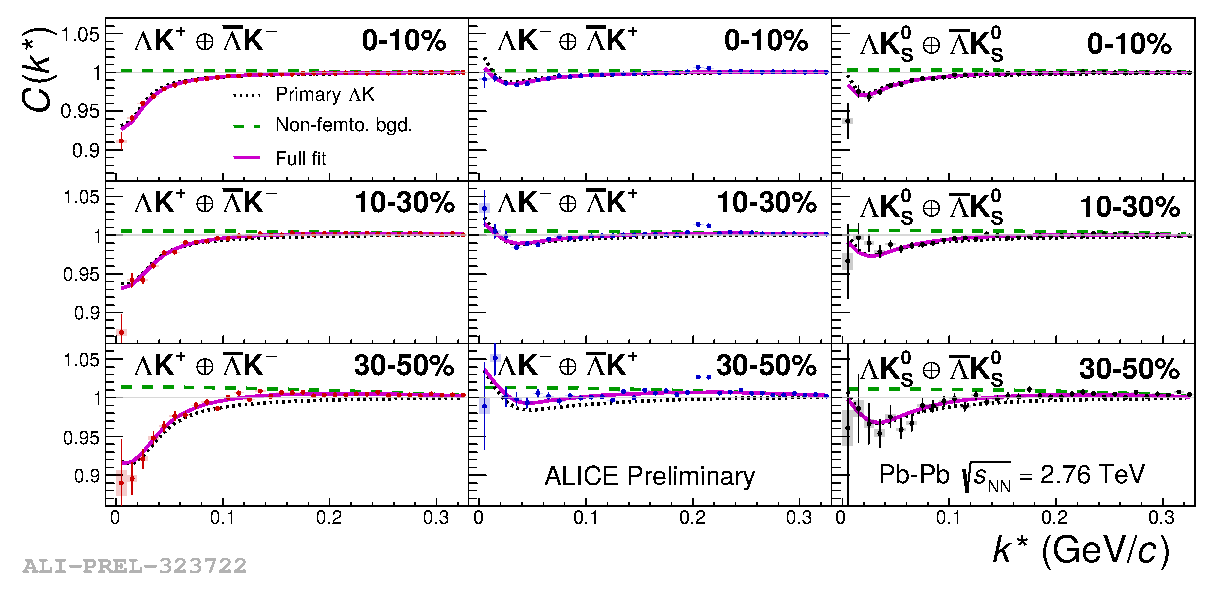
\includegraphics[width=\linewidth]{./Figures/Approved/OtherFormats/EPS/2019-06-11-canKStarCfwFits_CombineConj_AllAn_LabelLines.eps}
  \caption[\LamK data with fits]
  {
  (Color online) Fit results for the \LamK data, with pair and conjugate combined.
  The \LamKchP$\oplus$\ALamKchM data are shown in the left column, the \LamKchM$\oplus$\ALamKchP in the middle, and the \LamKs$\oplus$\ALamKs in the right. 
  Rows differentiate the different centrality intervals (0--10\% in the top, 10--30\% in the middle, and 30--50\% in the bottom).
  Lines represent statistical uncertainties, while boxes represent systematic uncertainties.
  The dotted curve shows the primary (\LamK) contribution to the fit, the dashed curve shows the fit to the non-femtoscopic background, and the solid curve shows the final fit.
 }
  \label{fig:LamKFits_3Res}
\end{figure}

\begin{figure}[h]
  \centering
  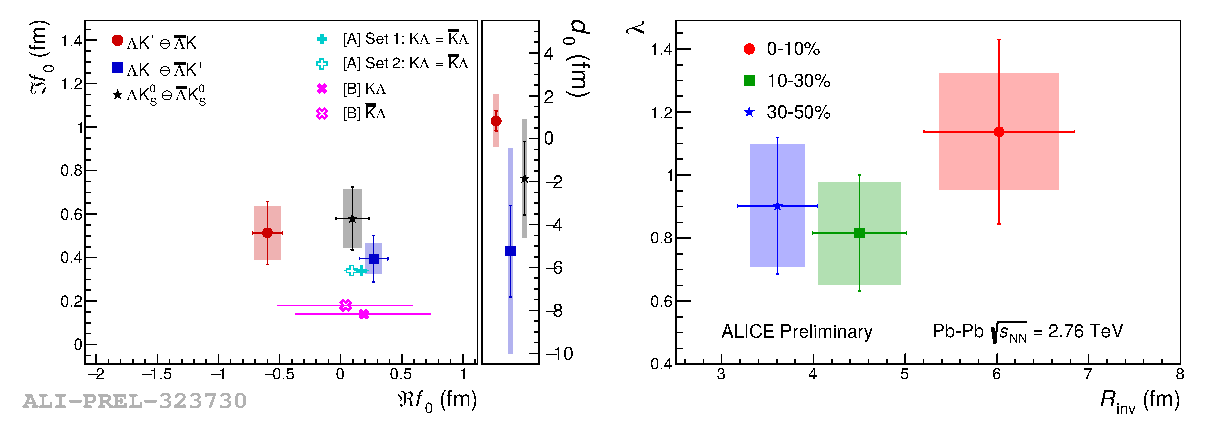
\includegraphics[width=\textwidth]{./Figures/Approved/OtherFormats/EPS/2019-06-11-FinalResults_Comp3An.eps}
  \caption[Extracted Scattering Parameters]
  {
  (Color online) Extracted fit parameters for all of the \LamK systems.  
  (Left) The scattering parameters, $\Im f_{0}$ and $\Re f_{0}$, together with $d_{0}$ to the right, for the \LamKchP (circles), \LamKchM (squares) and \LamKs (stars) systems.  
  (Right) The $\lambda_{\mathrm{Fit}}$ and radius parameters for the 0--10\% (circles), 10--30\% (squares), and 30--50\% (stars) centrality intervals.  
  In the fit, all \LamK systems share common radii.
  The cross~\cite{Liu:2006xja} and X~\cite{Mai:2009ce} points show theoretical predictions made using chiral perturbation theory.
  }
  \label{fig:ScattParams_3Res}
\end{figure}

Figure~\ref{fig:ScattParams_3Res} (left) summarizes the extracted \LamK scattering parameters, and includes theoretical predictions made using chiral perturbation theory~\cite{Liu:2006xja,Mai:2009ce}.
For all \LamK systems, positive imaginary parts of the scattering lengths, $\Im(f_{0})$, are extracted from the experimental data. 
This is expected, as $\Im(f_{0})$ describes the inelastic scattering channels.
More interestingly, the results show that the \LamKchP and \LamKchM systems differ in the sign of the real part, $\Re(f_{0})$, of their scattering lengths, with a negative value for \LamKchP and positive value for \LamKchM.
The $\Re f_{0}$ extracted for the \LamKs system is positive, and within uncertainties of that of the \LamKchM. 
The real part of the scattering length describes the effect of the strong interaction, making the difference in these systems quite intriguing.
As is the usual convention in femtoscopy, a positive $\Re(f_{0})$ signifies that the effect of the interaction is attractive, while a negative $\Re(f_{0})$ signifies a repulsive interaction.
Therefore, the femtoscopic signals from this analysis demonstrate that the strong interaction acts repulsively in the \LamKchP system, and acts attractively in the \LamKchM and \LamKs systems.

In Fig.~\ref{fig:ScattParams_3Res} (left), the predictions of~\cite{Liu:2006xja} do not distinguish the K\Lam and K\ALam interactions and results are shown for two different parameter sets, whereas~\cite{Mai:2009ce} offers unique K\Lam and $\overline{\mathrm{K}}$\Lam scattering parameters for a single parameter set. 
In all cases, the predicted scattering parameters have both positive real and imaginary components, which is clearly inconsistent with the \LamKchP system.
Past studies of kaon-proton scattering found the K$^{-}$--p interaction to be attractive, and that of the K$^{+}$--p to be repulsive~\cite{Humphrey:1962zz,Hadjimichef:2002xe,Ikeda:2012au}.
With respect to the kaons, this is similar to the current finding of an attractive \Lam--\KchM interaction and a repulsive \Lam--\KchP interaction.
This difference could be due to an effect arising from different quark--antiquark interactions between the pairs ($\rm s\overline{s}$ in \LamKchP, $\rm u\overline{u}$ in \LamKchM).
A related explanation could be that the effect is due to the different net strangeness for each system.
The quark content of the \Lam (\ALam) is uds ($\overline{\mathrm{uds}}$), that of the \KchP (\KchM) is u$\overline{\mathrm{s}}$ ($\overline{\mathrm{u}}$s), and the \Ks is a mixture of the neutral $\mathrm{K}^{0}$ and $\overline{\mathrm{K}^{0}}$ states with quark content $\frac{1}{\sqrt{2}}\left[\mathrm{d\overline{s} + \overline{d}s}\right]$.
It is interesting to note the presence of a $\mathrm{s\overline{s}}$ pair in the \LamKchP system contrasted with a $\mathrm{u\overline{u}}$ pair in the \LamKchM system.
Additionally, although the \Ks is a type average of \KchP and \KchM in some respects (e.g., electrically), it contains (anti)down quarks, whereas the \Kpm contain (anti)up quarks.


Figure~\ref{fig:ScattParams_3Res} (right) presents the $\lambda_{\mathrm{Fit}}$ and radius parameters for all three studied centrality percentile ranges.
The $\lambda_{\mathrm{Fit}}$ parameters are expected to be close to unity. 
The radii are observed to increase for more central events, as expected from a simple geometric picture of the collisions.


%************************************************************************************************************************
%************************************************************************************************************************
\section{Summary}
\label{sec:Summary}

\subfile{\ResultsDirBaseLamKch\SaveNameModLamKch/Tables/ResultsTableTriple_Vert.tex}

Results from a femtoscopic analysis of \LamK correlations in Pb--Pb collisions at $\sqrt{s_{\mathrm{NN}}}$ = 2.76 TeV measured by the ALICE experiment at the LHC have been presented, and are summarized in Table~\ref{tab:FitResultsLamK_3Res}.
The femtoscopic radii, $\lambda$ parameters, and scattering parameters were extracted from one-dimensional correlation functions in terms of the invariant momentum difference.
The scattering parameters of \LamK pairs in all three charge combinations (\LamKchP, \LamKchM, and \LamKs) have been measured for the first time.
Striking differences are observed in the \LamKchP, \LamKchM, and \LamKs correlation functions, which are reflected in the unique set of scattering parameters extracted for each.
The extracted scattering parameters indicate that the strong force is repulsive in the \LamKchP interaction and attractive in the \LamKchM and \LamKs interactions.
This effect could be due to different quark--antiquark interactions between the pairs, or from different net strangeness for each system. 
The non-femtoscopic background is found to result almost entirely from collective effects, and is described quantitatively with unprecedented precision with the THERMINATOR 2 event generator.
Finally, the \LamK systems exhibit source radii larger than expected from extrapolation from identical particle femtoscopic studies.
This effect is interpreted as resulting from the separation in space--time of the single-particle \Lam and K source distributions (i.e., the emission asymmetry of the source).
%\clearpage

%%%%% acknowledgements
\newenvironment{acknowledgement}{\relax}{\relax}
\begin{acknowledgement}
\section*{Acknowledgements}
%\input{acknowledgements.tex}    %%%%%%% done by webmaster team
\end{acknowledgement}

%%%%%%%% Bibliography (In case of using bibtex generate the bbl requested by arXiv)
\bibliographystyle{./styles/bibtex/splncs03_unsrt.bst}   % Remember we use title in the biblio
\bibliography{LamK_bibfile}
%\input {bibliography.tex}  

%%%%%%%%% appendix with author list
\newpage
\appendix
%
%% Following lines needed so, for instance, Fig D.1(a) not printed as simply 1(a) when referenced
\renewcommand{\thesubfigure}{\thefigure(\alph{subfigure})}
\makeatletter
\renewcommand{\p@subfigure}{}
\renewcommand{\@thesubfigure}{(\alph{subfigure})\hskip\subfiglabelskip}
%\input{}               %%%%%%%%%%% put your appendices here
%


%************************************************************************************************************************



\end{document}
